% !TEX TS-program = pdflatex
\documentclass[11pt]{article}

% -------------------- Packages --------------------
\usepackage[a4paper,margin=1in]{geometry}
\usepackage{amsmath,amssymb}
\usepackage[T1]{fontenc}
\usepackage{lmodern}
\usepackage{xcolor}
\usepackage{tcolorbox}
\tcbuselibrary{skins,breakable}
\usepackage{enumitem}
\usepackage{hyperref}

% --- Tables & Diagrams ---
\usepackage{booktabs}
\usepackage{array}
\usepackage{colortbl}
\usepackage{tikz}
\usepackage{pgfplots}
\pgfplotsset{compat=1.18}

\pagestyle{empty}

% -------------------- Dark Theme Colors --------------------
\definecolor{bg}{HTML}{000000}
\definecolor{pairbg}{HTML}{121212}
\definecolor{solbg}{HTML}{0A0A0A}
\definecolor{border}{HTML}{2A2A2A}
\definecolor{text}{HTML}{FFFFFF}
\definecolor{muted}{HTML}{C9CDD3}
\definecolor{gold}{HTML}{FFD700}
\definecolor{green}{HTML}{4ADE80}
\definecolor{cyan}{HTML}{38BDF8}

\definecolor{tablehead}{HTML}{1B1B1B}
\definecolor{tablerow}{HTML}{101010}

\pagecolor{bg}
\color{text}

\hypersetup{
  colorlinks=true,
  linkcolor=cyan,
  urlcolor=cyan
}

\setlength{\parindent}{0pt}
\setlength{\parskip}{10pt}

\setlist[itemize]{left=1.4em,itemsep=6pt,topsep=6pt}
\setlist[enumerate]{left=1.6em,itemsep=4pt,topsep=4pt}

% -------------------- tcolorbox Base --------------------
\tcbset{
  enhanced,
  breakable,
  arc=12pt,
  boxrule=0.8pt,
  left=16pt,right=16pt,top=12pt,bottom=12pt
}

\newtcolorbox{QAPair}[1]{%
  colback=pairbg,
  colbacklower=solbg,
  colframe=border,
  coltext=text,
  title=\textcolor{gold}{\bfseries #1},
  fonttitle=\bfseries,
  coltitle=text,
  segmentation style={draw=border, dashed, line width=0.6pt},
}

\newtcolorbox{QuickBox}{%
  colback=pairbg,
  colframe=cyan,
  coltext=text,
  fontupper=\color{text},
  borderline north={4pt}{0pt}{cyan},
  arc=14pt,
  boxrule=0.8pt
}

% Helper for step headings
\newcommand{\Step}[1]{\textcolor{muted}{\textbf{Step #1:}}}

% -------------------- pgfplots dark styling --------------------
\pgfplotsset{
  every axis/.append style={
    axis line style={color=text},
    tick style={color=text},
    ticklabel style={color=text},
    label style={color=text},
    title style={color=text},
    grid style={color=border},
    legend style={draw=border, fill=pairbg, text=text},
  }
}

% A small helper to format tables nicely on dark background
\newcommand{\DarkTable}{%
  \rowcolors{2}{tablerow}{solbg}
  \renewcommand{\arraystretch}{1.2}
  \setlength{\tabcolsep}{10pt}
}

% ============================================================
\begin{document}

\begin{center}
{\LARGE\bfseries \textcolor{gold}{Exercise 11.2 --- Solutions}}\\[-2pt]
\end{center}

\begin{QuickBox}
{\color{cyan}\bfseries Must-know formulas + techniques}\par\medskip
\begin{itemize}
\item \textbf{Arithmetic mean (simple list):}
\[
\bar{x}=\frac{\sum x}{n}.
\]
\textbf{Technique:} add all values $\to$ count how many values ($n$) $\to$ divide.

\item \textbf{Mean from a frequency table (grouped data):}
\[
\bar{x}=\frac{\sum (f\cdot x)}{\sum f},
\]
where $x$ is the \textbf{class mark} (midpoint).

\item \textbf{Class mark (midpoint):}
\[
x=\frac{\text{lower limit}+\text{upper limit}}{2}.
\]

\item \textbf{Weighted mean:}
\[
\bar{x}_w=\frac{\sum (w\cdot x)}{\sum w}.
\]
\textbf{Technique:} multiply each value by its weight $\to$ add $\to$ divide by total weights.

\item \textbf{Median (simple list):}
\textbf{Technique:} sort the data.
Odd $n$: median is middle value.  
Even $n$: median is average of the two middle values.

\item \textbf{Median (grouped data):}
\[
\text{Median}=L+\Bigl(\frac{\frac{N}{2}-\text{CF}_{\text{prev}}}{f}\Bigr)h.
\]
\textbf{Where:} $L$=lower boundary of median class, $N=\sum f$, $h$=class width, $f$=frequency of median class.

\item \textbf{Mode (simple list):} value with the highest frequency (most repeated).  
If all frequencies are the same $\Rightarrow$ \textbf{no mode}.

\item \textbf{Mode (grouped data):}
\[
\text{Mode}=L+\Bigl(\frac{f_1-f_0}{2f_1-f_0-f_2}\Bigr)h
\]
($f_1$=modal class frequency, $f_0$=previous, $f_2$=next).
\end{itemize}
\end{QuickBox}

% ============================================================
% Q1 (separate boxes)
\begin{QAPair}{Question 1 (i)}
\textcolor{gold}{\bfseries Question:} Find mean of $x=2,4,6,8,10,12$.
\tcblower
\textcolor{green}{\bfseries Answer:}
\[
\begin{aligned}
\Step{1}\;& \text{Add all values: } \sum x=2+4+6+8+10+12=42.\\
\Step{2}\;& \text{Count values: } n=6.\\
\Step{3}\;& \bar{x}=\frac{\sum x}{n}=\frac{42}{6}=7.
\end{aligned}
\]
\end{QAPair}

\begin{QAPair}{Question 1 (ii)}
\textcolor{gold}{\bfseries Question:} Find mean of $y=3,4,-1,7,-8,-5,0$.
\tcblower
\textcolor{green}{\bfseries Answer:}
\[
\begin{aligned}
\Step{1}\;& \sum y=3+4-1+7-8-5+0=0.\\
\Step{2}\;& n=7.\\
\Step{3}\;& \bar{y}=\frac{0}{7}=0.
\end{aligned}
\]
\end{QAPair}

\begin{QAPair}{Question 1 (iii)}
\textcolor{gold}{\bfseries Question:} Find mean of $z=0,4,8,12,16,20,24,28$.
\tcblower
\textcolor{green}{\bfseries Answer:}
\[
\begin{aligned}
\Step{1}\;& \sum z=0+4+8+12+16+20+24+28=112.\\
\Step{2}\;& n=8.\\
\Step{3}\;& \bar{z}=\frac{112}{8}=14.
\end{aligned}
\]
\end{QAPair}

\begin{QAPair}{Question 1 (iv)}
\textcolor{gold}{\bfseries Question:} Find mean of $u=3.1,4.2,5.3,6.4,7.5,8.6,9.7,10.8$.
\tcblower
\textcolor{green}{\bfseries Answer:}
\[
\begin{aligned}
\Step{1}\;& \sum u=3.1+4.2+5.3+6.4+7.5+8.6+9.7+10.8=55.6.\\
\Step{2}\;& n=8.\\
\Step{3}\;& \bar{u}=\frac{55.6}{8}=6.95.
\end{aligned}
\]
\end{QAPair}

\begin{QAPair}{Question 1 (v)}
\textcolor{gold}{\bfseries Question:} Find mean of $v=5,5,5,5,5,5,5,5$.
\tcblower
\textcolor{green}{\bfseries Answer:}
\[
\Step{1}\; \text{All values are the same (5), so the mean is also } \boxed{5}.
\]
\end{QAPair}

% ============================================================
% Q2
\begin{QAPair}{Question 2}
\textcolor{gold}{\bfseries Question:} Scores of two batsmen A and B are: \\
$A: 12,15,6,73,7,19,199,36,84,29$ \\
$B: 47,12,76,48,4,51,37,48,13,0$ \\
Find mean of both and state who is better.
\tcblower
\textcolor{green}{\bfseries Answer:}

\textcolor{muted}{\textbf{Technique:} add all scores $\to$ divide by number of innings ($n=10$).}

\textcolor{gold}{\bfseries Player A}
\[
\begin{aligned}
\Step{1}\;& \sum A=12+15+6+73+7+19+199+36+84+29=480.\\
\Step{2}\;& n=10.\\
\Step{3}\;& \bar{A}=\frac{480}{10}=48.
\end{aligned}
\]

\textcolor{gold}{\bfseries Player B}
\[
\begin{aligned}
\Step{1}\;& \sum B=47+12+76+48+4+51+37+48+13+0=336.\\
\Step{2}\;& n=10.\\
\Step{3}\;& \bar{B}=\frac{336}{10}=33.6.
\end{aligned}
\]

\textcolor{gold}{\bfseries Conclusion:}\;
Since $48>33.6$, \textbf{Player A} is better as a run getter.
\end{QAPair}

% ============================================================
% Q3 (easier explanation)
\begin{QAPair}{Question 3}
\textcolor{gold}{\bfseries Question:} Marks of four students with subject weights are given. Find weighted mean of marks of each student.\\[4pt]
\begin{center}
\DarkTable
\begin{tabular}{>{\bfseries}l c c c c c}
\rowcolor{tablehead}\textcolor{text}{Subject} & \textcolor{text}{Weight} &
\textcolor{text}{Hanzala} & \textcolor{text}{Musa} & \textcolor{text}{Zaki} & \textcolor{text}{Saleh}\\
Mathematics & 4 & 70 & 80 & 90 & 95\\
Physics     & 3 & 95 & 60 & 55 & 70\\
Chemistry   & 2 & 80 & 65 & 50 & 60\\
Biology     & 1 & 55 & 45 & 65 & 60\\
\end{tabular}
\end{center}
\tcblower
\textcolor{green}{\bfseries Answer:}

\textcolor{muted}{\textbf{Idea (easy):} A subject with higher weight counts more.\\
\textbf{Steps:} (1) Multiply each mark by its weight. (2) Add them. (3) Divide by total weight.}

\[
\Step{1}\; \sum w=4+3+2+1=10.
\]

\textcolor{gold}{\bfseries Hanzala}
\[
\begin{aligned}
\Step{1}\;& 70(4)=280,\; 95(3)=285,\; 80(2)=160,\; 55(1)=55.\\
\Step{2}\;& \sum wx=280+285+160+55=780.\\
\Step{3}\;& \bar{x}_w=\frac{780}{10}=78.
\end{aligned}
\]

\textcolor{gold}{\bfseries Musa}
\[
\begin{aligned}
\Step{1}\;& 80(4)=320,\; 60(3)=180,\; 65(2)=130,\; 45(1)=45.\\
\Step{2}\;& \sum wx=320+180+130+45=675.\\
\Step{3}\;& \bar{x}_w=\frac{675}{10}=67.5.
\end{aligned}
\]

\textcolor{gold}{\bfseries Zaki}
\[
\begin{aligned}
\Step{1}\;& 90(4)=360,\; 55(3)=165,\; 50(2)=100,\; 65(1)=65.\\
\Step{2}\;& \sum wx=360+165+100+65=690.\\
\Step{3}\;& \bar{x}_w=\frac{690}{10}=69.
\end{aligned}
\]

\textcolor{gold}{\bfseries Saleh}
\[
\begin{aligned}
\Step{1}\;& 95(4)=380,\; 70(3)=210,\; 60(2)=120,\; 60(1)=60.\\
\Step{2}\;& \sum wx=380+210+120+60=770.\\
\Step{3}\;& \bar{x}_w=\frac{770}{10}=77.
\end{aligned}
\]

\textcolor{gold}{\bfseries Final answers:}\;
Hanzala $=78$, Musa $=67.5$, Zaki $=69$, Saleh $=77$.
\end{QAPair}

% ============================================================
% Q4 (easier + table + diagram)
\begin{QAPair}{Question 4}
\textcolor{gold}{\bfseries Question:} Frequency distribution (distance classes). Find arithmetic mean.\\[4pt]
\begin{center}
\DarkTable
\begin{tabular}{>{\bfseries}c c c c c}
\rowcolor{tablehead}\textcolor{text}{Class intervals} &
\textcolor{text}{0--5} & \textcolor{text}{5--10} & \textcolor{text}{10--15} & \textcolor{text}{15--20} & \textcolor{text}{20--25}\\
\textcolor{text}{Frequencies $f$} & 5 & 7 & 10 & 6 & 2\\
\end{tabular}
\end{center}
\tcblower
\textcolor{green}{\bfseries Answer:}

\textcolor{muted}{\textbf{Technique for grouped mean:}\\
(1) Find class mark $x$ for each class. (2) Compute $fx$. (3) Mean $=\dfrac{\sum fx}{\sum f}$.}

\begin{center}
\DarkTable
\begin{tabular}{>{\bfseries}c c c}
\rowcolor{tablehead}\textcolor{text}{Class} & \textcolor{text}{Class mark $x$} & \textcolor{text}{$fx$}\\
0--5   & $\frac{0+5}{2}=2.5$  & $5(2.5)=12.5$\\
5--10  & $\frac{5+10}{2}=7.5$ & $7(7.5)=52.5$\\
10--15 & $\frac{10+15}{2}=12.5$ & $10(12.5)=125$\\
15--20 & $\frac{15+20}{2}=17.5$ & $6(17.5)=105$\\
20--25 & $\frac{20+25}{2}=22.5$ & $2(22.5)=45$\\
\rowcolor{tablehead}\textcolor{text}{Total} & \textcolor{text}{$\sum f=30$} & \textcolor{text}{$\sum fx=340$}\\
\end{tabular}
\end{center}

\[
\Step{1}\; \bar{x}=\frac{\sum fx}{\sum f}=\frac{340}{30}=11.333\ldots \approx \boxed{11.33}.
\]

\textcolor{gold}{\bfseries Diagram (histogram; equal widths)}\\
\begin{center}
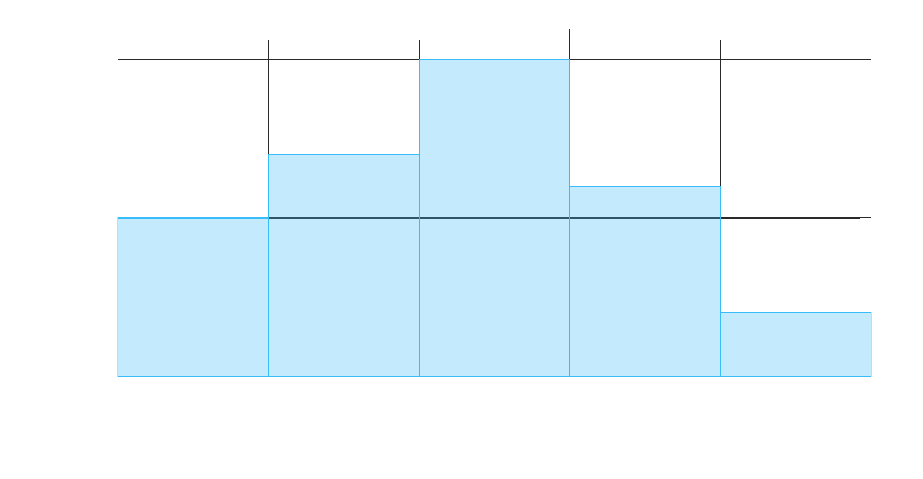
\begin{tikzpicture}
\begin{axis}[
  width=0.92\linewidth,
  height=6.0cm,
  ymin=0, ymax=11,
  xmin=0, xmax=25,
  grid=both,
  xlabel={Distance class},
  ylabel={Frequency},
  xtick={0,5,10,15,20,25},
]
\addplot+[ybar interval, draw=cyan, fill=cyan, fill opacity=0.30, mark=no]
coordinates {(0,5) (5,7) (10,10) (15,6) (20,2) (25,0)};
\end{axis}
\end{tikzpicture}
\end{center}
\end{QAPair}

% ============================================================
% Q5 (easier + table + diagram)
\begin{QAPair}{Question 5}
\textcolor{gold}{\bfseries Question:} Detergent packs sold against mass (kg). Find arithmetic mean.\\[4pt]
\begin{center}
\DarkTable
\begin{tabular}{>{\bfseries}c c c c c}
\rowcolor{tablehead}\textcolor{text}{Classes (kg)} &
\textcolor{text}{1--9} & \textcolor{text}{10--18} & \textcolor{text}{19--27} & \textcolor{text}{28--36} & \textcolor{text}{37--45}\\
\textcolor{text}{No. of packs $f$} & 10 & 15 & 18 & 15 & 12\\
\end{tabular}
\end{center}
\tcblower
\textcolor{green}{\bfseries Answer:}

\textcolor{muted}{Same grouped-mean steps: class mark $x$ $\to$ compute $fx$ $\to$ mean $=\dfrac{\sum fx}{\sum f}$.}

\begin{center}
\DarkTable
\begin{tabular}{>{\bfseries}c c c}
\rowcolor{tablehead}\textcolor{text}{Class} & \textcolor{text}{Class mark $x$} & \textcolor{text}{$fx$}\\
1--9   & $\frac{1+9}{2}=5$   & $10(5)=50$\\
10--18 & $\frac{10+18}{2}=14$ & $15(14)=210$\\
19--27 & $\frac{19+27}{2}=23$ & $18(23)=414$\\
28--36 & $\frac{28+36}{2}=32$ & $15(32)=480$\\
37--45 & $\frac{37+45}{2}=41$ & $12(41)=492$\\
\rowcolor{tablehead}\textcolor{text}{Total} & \textcolor{text}{$\sum f=70$} & \textcolor{text}{$\sum fx=1646$}\\
\end{tabular}
\end{center}

\[
\Step{1}\; \bar{x}=\frac{1646}{70}=23.514\ldots \approx \boxed{23.51\text{ kg}}.
\]

\textcolor{gold}{\bfseries Diagram (histogram; equal widths)}\\
\begin{center}
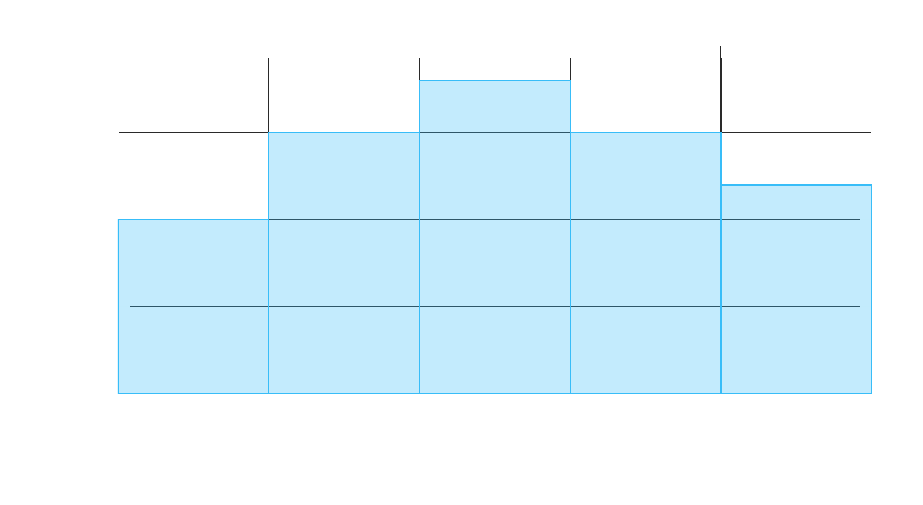
\begin{tikzpicture}
\begin{axis}[
  width=0.92\linewidth,
  height=6.0cm,
  ymin=0, ymax=20,
  xmin=1, xmax=46,
  grid=both,
  xlabel={Mass class (kg)},
  ylabel={No. of packs},
  xtick={1,10,19,28,37,46},
]
\addplot+[ybar interval, draw=cyan, fill=cyan, fill opacity=0.30, mark=no]
coordinates {(1,10) (10,15) (19,18) (28,15) (37,12) (46,0)};
\end{axis}
\end{tikzpicture}
\end{center}
\end{QAPair}

% ============================================================
% Q6 (separate boxes)
\begin{QAPair}{Question 6 (i)}
\textcolor{gold}{\bfseries Question:} Find median of $1,4,2,5,3,7,6$.
\tcblower
\textcolor{green}{\bfseries Answer:}
\[
\begin{aligned}
\Step{1}\;& \text{Sort: } 1,2,3,4,5,6,7.\\
\Step{2}\;& n=7 \text{ (odd), so median is the middle (4th) value.}\\
\Step{3}\;& \text{Median}=\boxed{4}.
\end{aligned}
\]
\end{QAPair}

\begin{QAPair}{Question 6 (ii)}
\textcolor{gold}{\bfseries Question:} Find median of $\pm2,\pm4,\pm6,\pm8$.
\tcblower
\textcolor{green}{\bfseries Answer:}
\[
\begin{aligned}
\Step{1}\;& \text{Write all values: } -2,2,-4,4,-6,6,-8,8.\\
\Step{2}\;& \text{Sort: } -8,-6,-4,-2,2,4,6,8.\\
\Step{3}\;& n=8 \text{ (even), median is average of 4th and 5th.}\\
\Step{4}\;& \text{Median}=\frac{-2+2}{2}=0 \Rightarrow \boxed{0}.
\end{aligned}
\]
\end{QAPair}

\begin{QAPair}{Question 6 (iii)}
\textcolor{gold}{\bfseries Question:} Find median of $0,1,-2,-3,4,5,6,3$.
\tcblower
\textcolor{green}{\bfseries Answer:}
\[
\begin{aligned}
\Step{1}\;& \text{Sort: } -3,-2,0,1,3,4,5,6.\\
\Step{2}\;& n=8 \text{ (even), median is average of 4th and 5th.}\\
\Step{3}\;& \text{Median}=\frac{1+3}{2}=2 \Rightarrow \boxed{2}.
\end{aligned}
\]
\end{QAPair}

\begin{QAPair}{Question 6 (iv)}
\textcolor{gold}{\bfseries Question:} Find median of $4,3,1,-3,2,-3,3,4,1$.
\tcblower
\textcolor{green}{\bfseries Answer:}
\[
\begin{aligned}
\Step{1}\;& \text{Sort: } -3,-3,1,1,2,3,3,4,4.\\
\Step{2}\;& n=9 \text{ (odd), median is middle (5th) value.}\\
\Step{3}\;& \text{Median}=\boxed{2}.
\end{aligned}
\]
\end{QAPair}

\begin{QAPair}{Question 6 (v)}
\textcolor{gold}{\bfseries Question:} Find median of $4,4,4,4,4,4$.
\tcblower
\textcolor{green}{\bfseries Answer:}
\[
\Step{1}\; \text{All values are }4,\ \text{so the median is } \boxed{4}.
\]
\end{QAPair}

% ============================================================
% Q7
\begin{QAPair}{Question 7}
\textcolor{gold}{\bfseries Question:} Radii (cm) and frequencies are given. Find the median radius.\\[4pt]
\begin{center}
\DarkTable
\begin{tabular}{>{\bfseries}c c c c c c c c c}
\rowcolor{tablehead}\textcolor{text}{Radius (cm)} &
0.2 & 0.4 & 0.6 & 0.8 & 1.0 & 1.2 & 1.4 & 1.6 & 1.8\\
\textcolor{text}{Frequency $f$} &
5 & 7 & 13 & 20 & 33 & 24 & 15 & 9 & 6\\
\end{tabular}
\end{center}
\tcblower
\textcolor{green}{\bfseries Answer:}

\textcolor{muted}{\textbf{Technique:} Find total $N$, locate the middle positions, then use cumulative frequency (CF).}

\[
\Step{1}\; N=\sum f=132 \Rightarrow \text{median positions are } 66\text{th and }67\text{th}.
\]

\begin{center}
\DarkTable
\begin{tabular}{>{\bfseries}c c c}
\rowcolor{tablehead}\textcolor{text}{Radius} & \textcolor{text}{$f$} & \textcolor{text}{CF}\\
0.2 & 5  & 5\\
0.4 & 7  & 12\\
0.6 & 13 & 25\\
0.8 & 20 & 45\\
1.0 & 33 & 78\\
1.2 & 24 & 102\\
1.4 & 15 & 117\\
1.6 & 9  & 126\\
1.8 & 6  & 132\\
\end{tabular}
\end{center}

\[
\Step{2}\; 45<66,67\le 78 \Rightarrow \text{both positions fall at radius } 1.0.
\]
\[
\Step{3}\; \boxed{\text{Median radius}=1.0\text{ cm}}.
\]
\end{QAPair}

% ============================================================
% Q8
\begin{QAPair}{Question 8}
\textcolor{gold}{\bfseries Question:} Old age house data: classes $40$--$50,50$--$60,60$--$70,70$--$80,80$--$90$ with $f=3,8,11,5,4$. Find median age.
\tcblower
\textcolor{green}{\bfseries Answer:}

\textcolor{muted}{\textbf{Technique (grouped median):}
(1) Make CF. (2) Find median class using $N/2$. (3) Apply formula.}

\begin{center}
\DarkTable
\begin{tabular}{>{\bfseries}c c c}
\rowcolor{tablehead}\textcolor{text}{Class interval} & \textcolor{text}{Frequency $f$} & \textcolor{text}{CF}\\
40--50 & 3  & 3\\
50--60 & 8  & 11\\
60--70 & 11 & 22\\
70--80 & 5  & 27\\
80--90 & 4  & 31\\
\rowcolor{tablehead}\textcolor{text}{Total} & \textcolor{text}{\bfseries 31} & \textcolor{text}{ }\\
\end{tabular}
\end{center}

\[
\Step{1}\; N=31 \Rightarrow \frac{N}{2}=15.5.
\]
\[
\Step{2}\; 11<15.5\le 22 \Rightarrow \text{median class is } 60\text{--}70.
\]
\[
\Step{3}\; L=59.5,\ h=10,\ f=11,\ \text{CF}_{\text{prev}}=11.
\]
\[
\Step{4}\; \text{Median}=L+\Bigl(\frac{\frac{N}{2}-\text{CF}_{\text{prev}}}{f}\Bigr)h
=59.5+\Bigl(\frac{15.5-11}{11}\Bigr)10
\approx 63.6.
\]

\[
\boxed{\text{Median age}\approx 63.6\text{ years}}
\]
\end{QAPair}

% ============================================================
% Q9 (separate boxes)
\begin{QAPair}{Question 9 (i)}
\textcolor{gold}{\bfseries Question:} Find mode of $1,2,3,4,5,6$.
\tcblower
\textcolor{green}{\bfseries Answer:}
\[
\begin{aligned}
\Step{1}\;& \text{Mode = value that occurs most.}\\
\Step{2}\;& \text{Here each value occurs once.}\\
\Step{3}\;& \boxed{\text{No mode}}.
\end{aligned}
\]
\end{QAPair}

\begin{QAPair}{Question 9 (ii)}
\textcolor{gold}{\bfseries Question:} Find mode of $2,4,2,3,2,5,3,2,5,4,2$.
\tcblower
\textcolor{green}{\bfseries Answer:}
\[
\begin{aligned}
\Step{1}\;& \text{Count repeats: } 2 \text{ occurs }5 \text{ times (highest).}\\
\Step{2}\;& \boxed{\text{Mode}=2}.
\end{aligned}
\]
\end{QAPair}

\begin{QAPair}{Question 9 (iii)}
\textcolor{gold}{\bfseries Question:} Find mode of $120,130,140,225,125,225,120$.
\tcblower
\textcolor{green}{\bfseries Answer:}
\[
\begin{aligned}
\Step{1}\;& 120 \text{ occurs twice, } 225 \text{ occurs twice, others once.}\\
\Step{2}\;& \text{Highest frequency is }2 \text{ for both }120\text{ and }225.\\
\Step{3}\;& \boxed{\text{Bimodal: }120 \text{ and }225}.
\end{aligned}
\]
\end{QAPair}

\begin{QAPair}{Question 9 (iv)}
\textcolor{gold}{\bfseries Question:} Find mode of $2,4,3,5,5,3,4,2$.
\tcblower
\textcolor{green}{\bfseries Answer:}
\[
\begin{aligned}
\Step{1}\;& 2,3,4,5 \text{ each occurs twice.}\\
\Step{2}\;& \text{No single value occurs most.}\\
\Step{3}\;& \boxed{\text{No mode}}.
\end{aligned}
\]
\end{QAPair}

% ============================================================
% Q10
\begin{QAPair}{Question 10}
\textcolor{gold}{\bfseries Question:} Find mean, median and mode for:
\[
\begin{array}{c|cccccc}
x & 0 & 1 & 2 & 3 & 4 & 5\\ \hline
f & 3 & 5 & 9 & 4 & 2 & 1
\end{array}
\]
\tcblower
\textcolor{green}{\bfseries Answer:}

\textcolor{gold}{\bfseries (a) Mean}
\[
\begin{aligned}
\Step{1}\;& N=\sum f=3+5+9+4+2+1=24.\\
\Step{2}\;& \sum xf=0(3)+1(5)+2(9)+3(4)+4(2)+5(1)=48.\\
\Step{3}\;& \bar{x}=\frac{\sum xf}{\sum f}=\frac{48}{24}=2.
\end{aligned}
\]
So, \boxed{\text{Mean}=2}.

\textcolor{gold}{\bfseries (b) Median}
\[
\begin{aligned}
\Step{1}\;& N=24 \Rightarrow \text{median positions are }12\text{th and }13\text{th}.\\
\Step{2}\;& \text{CF: }3,8,17,21,23,24.\\
\Step{3}\;& 12\text{th and }13\text{th lie in CF }17 \Rightarrow x=2.
\end{aligned}
\]
So, \boxed{\text{Median}=2}.

\textcolor{gold}{\bfseries (c) Mode}
\[
\Step{1}\; \text{Highest frequency is }9 \text{ at } x=2 \Rightarrow \boxed{\text{Mode}=2}.
\]
\end{QAPair}

% ============================================================
% Q11 (separate boxes)
\begin{QAPair}{Question 11 (a)}
\textcolor{gold}{\bfseries Question:} Classes $1$--$4,5$--$8,9$--$12,13$--$16,17$--$20$ with $f=9,8,10,6,7$. Find modal value.
\tcblower
\textcolor{green}{\bfseries Answer:}

\textcolor{muted}{\textbf{Steps:}
(1) Modal class has greatest frequency. (2) Use mode formula for grouped data.}

\[
\Step{1}\; \text{Greatest frequency is }10 \Rightarrow \text{modal class } 9\text{--}12.
\]
Use continuous boundaries: $8.5$--$12.5$ so
\[
L=8.5,\quad h=4,\quad f_1=10,\quad f_0=8,\quad f_2=6.
\]
\[
\begin{aligned}
\Step{2}\;& \text{Mode}=L+\Bigl(\frac{f_1-f_0}{2f_1-f_0-f_2}\Bigr)h\\
&=8.5+\Bigl(\frac{10-8}{2(10)-8-6}\Bigr)4
=8.5+\Bigl(\frac{2}{6}\Bigr)4
\approx 9.83.
\end{aligned}
\]
\[
\boxed{\text{Mode}\approx 9.83}
\]
\end{QAPair}

\begin{QAPair}{Question 11 (b)}
\textcolor{gold}{\bfseries Question:} Classes $10$--$15,15$--$20,20$--$25,25$--$30,30$--$35$ with $f=7,6,3,2,1$. Find modal value.
\tcblower
\textcolor{green}{\bfseries Answer:}

\[
\Step{1}\; \text{Greatest frequency is }7 \Rightarrow \text{modal class } 10\text{--}15.
\]
Continuous boundaries: $9.5$--$14.5$ so $L=9.5$ and $h=5$.  
Here the previous class is not given, so we take $f_0=0$ (common textbook method). Also $f_2=6$.

\[
\begin{aligned}
\Step{2}\;& \text{Mode}=L+\Bigl(\frac{f_1-f_0}{2f_1-f_0-f_2}\Bigr)h\\
&=9.5+\Bigl(\frac{7-0}{2(7)-0-6}\Bigr)5
=9.5+\Bigl(\frac{7}{8}\Bigr)5
=13.875\approx 13.88.
\end{aligned}
\]
\[
\boxed{\text{Mode}\approx 13.88}
\]
\end{QAPair}

\end{document}
